\section{Experiments}
\label{sec:experiments}
\subsection{Dataset and common evaluation}
Waymo-405841~\cite{sun2020waymo} is a moving front-facing road sequence, Dl3dv-2~\cite{ling2024dl3dv} is an outdoor walk-through, and Re10k-1 is an indoor RealEstate10K sequence~\cite{zhou2018stereo}. We hold out every eighth image starting with index zero in natural filename order. We undistort Waymo with the supplied Brown--Conrady calibration and prepare it at $960\times640$ pixels. The other two scenes use $256\times256$ pixels. Table~\ref{tab:splits} gives exact counts. Sparse training retains original positions $1,1+k,1+2k,\dots$ with $k=10$ for Waymo and $k=30$ for the other sequences, skipping held-out IDs. The sparse experiment excludes unused training images from geometry initialization, optimization, and generation.

\begin{table}[t]
  \centering\small
  \begin{tabular}{lrrrr}
    \toprule
    Scene & Full & Sparse & Test & Stride \\
    \midrule
    Waymo-405841 & 174 & 20 & 25 & 10 \\
    Dl3dv-2 & 267 & 11 & 39 & 30 \\
    Re10k-1 & 244 & 10 & 35 & 30 \\
    \bottomrule
  \end{tabular}
  \caption{Fixed image splits and sparse sampling strides. Full and sparse reconstructions use identical held-out IDs.}
  \label{tab:splits}
\end{table}

We fit a single scene similarity transform from estimated training centers to the provided reference centers using Umeyama alignment~\cite{umeyama1991least}. We compute absolute trajectory error (ATE) as the root mean square center residual in reference trajectory units. Part 1 fits and scores on each initializer's complete training set, while Part 2 compares both conditions on the same sparse IDs. For rendering, each condition fits the reverse direction on all of its available real training centers and maps the held-out reference cameras into the reconstruction frame with reference intrinsics. We average PSNR, SSIM~\cite{wang2004ssim}, and AlexNet LPIPS~\cite{zhang2018lpips} across all held-out renders. No test imagery or test-pose refinement enters training. Camera parameters stay fixed throughout optimization, so ATE is constant during any continuation.

Part 1 ran on an RTX 4090 and Part 2 on a course RTX A6000, both using PyTorch 2.6.0 with CUDA 12.4 and gsplat 1.5.3. The distinct devices and memory strategies make wall-clock comparisons within each stage the appropriate comparison. All Part 1 and Part 2 comparisons use seed 42, 7,000 training iterations, and checkpoints at 500, 1,000, 2,000, 4,000, and 7,000 iterations. Intermediate test measurements describe convergence, and the prespecified 7,000-step state is the reported endpoint.

\subsection{Part 1: Dense geometry initialization}
\label{sec:part1}

\begin{table*}[!t]
  \centering\small
  \begin{tabular}{llrrrrrrr}
    \toprule
    Scene & Initializer & PSNR (dB) $\uparrow$ & SSIM $\uparrow$ & LPIPS $\downarrow$ &
    ATE $\downarrow$ & Init. (s) $\downarrow$ & Train (s) & Total (s) $\downarrow$ \\
    \midrule
    Waymo & COLMAP & 17.11 & 0.613 & \textbf{0.440} & \textbf{0.49078} & 805.8 & 186.9 & 1091.2 \\
          & VGGT & \textbf{17.74} & \textbf{0.655} & 0.521 & 0.92756 & 74.7 & 178.1 & 339.4 \\
          & VGGT-$\Omega$ & 16.56 & 0.624 & 0.505 & 0.60770 & \textbf{36.2} & 183.0 & \textbf{308.1} \\
    \midrule
    DL3DV & COLMAP & \textbf{23.61} & \textbf{0.771} & \textbf{0.077} & \textbf{0.01245} & 669.4 & 55.2 & 816.1 \\
          & VGGT & 18.52 & 0.513 & 0.195 & 0.03315 & 122.0 & 72.7 & 250.3 \\
          & VGGT-$\Omega$ & 20.10 & 0.661 & 0.181 & 0.01481 & \textbf{42.1} & 69.9 & \textbf{148.3} \\
    \midrule
    RealEstate10K & COLMAP & 11.07 & 0.276 & 0.392 & 0.01990 & 390.1 & 63.7 & 493.4 \\
                  & VGGT & 11.38 & 0.291 & 0.398 & 0.04512 & 109.6 & 85.0 & 259.6 \\
                  & VGGT-$\Omega$ & \textbf{18.33} & \textbf{0.640} & \textbf{0.068} & \textbf{0.00964} & \textbf{40.2} & 80.7 & \textbf{160.4} \\
    \bottomrule
  \end{tabular}
  \caption{Dense inputs, trained for 7,000 steps. ATE uses each scene's reference units. Initialization includes loading, pose and point estimation, and export. Total wall time includes all five test evaluations and artifact verification.}
  \label{tab:dense}
\end{table*}

\begin{figure*}[!t]
  \centering
  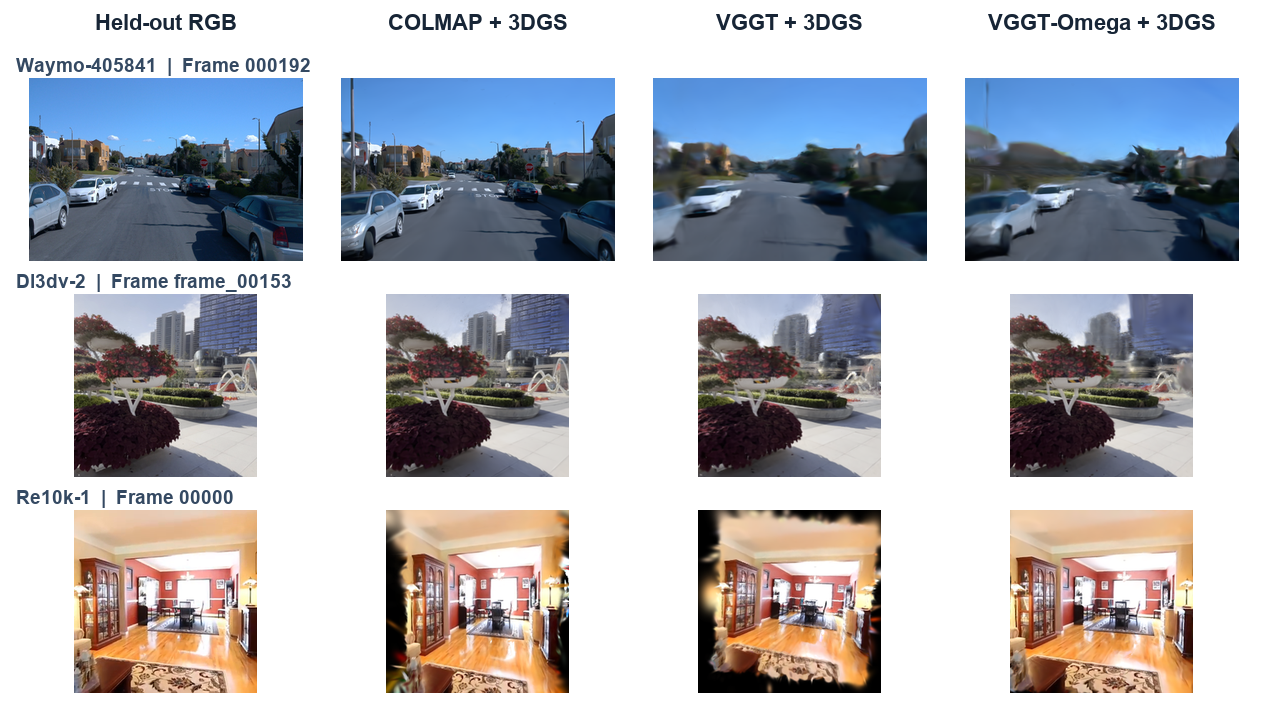
\includegraphics[width=0.94\textwidth]{part1_comparison.png}
  \caption{Example held-out images and the corresponding raw 3DGS renders from the three candidate initializers. Each row uses the same target camera across methods.}
  \label{fig:dense_qual}
\end{figure*}

\begin{figure*}[!t]
  \centering
  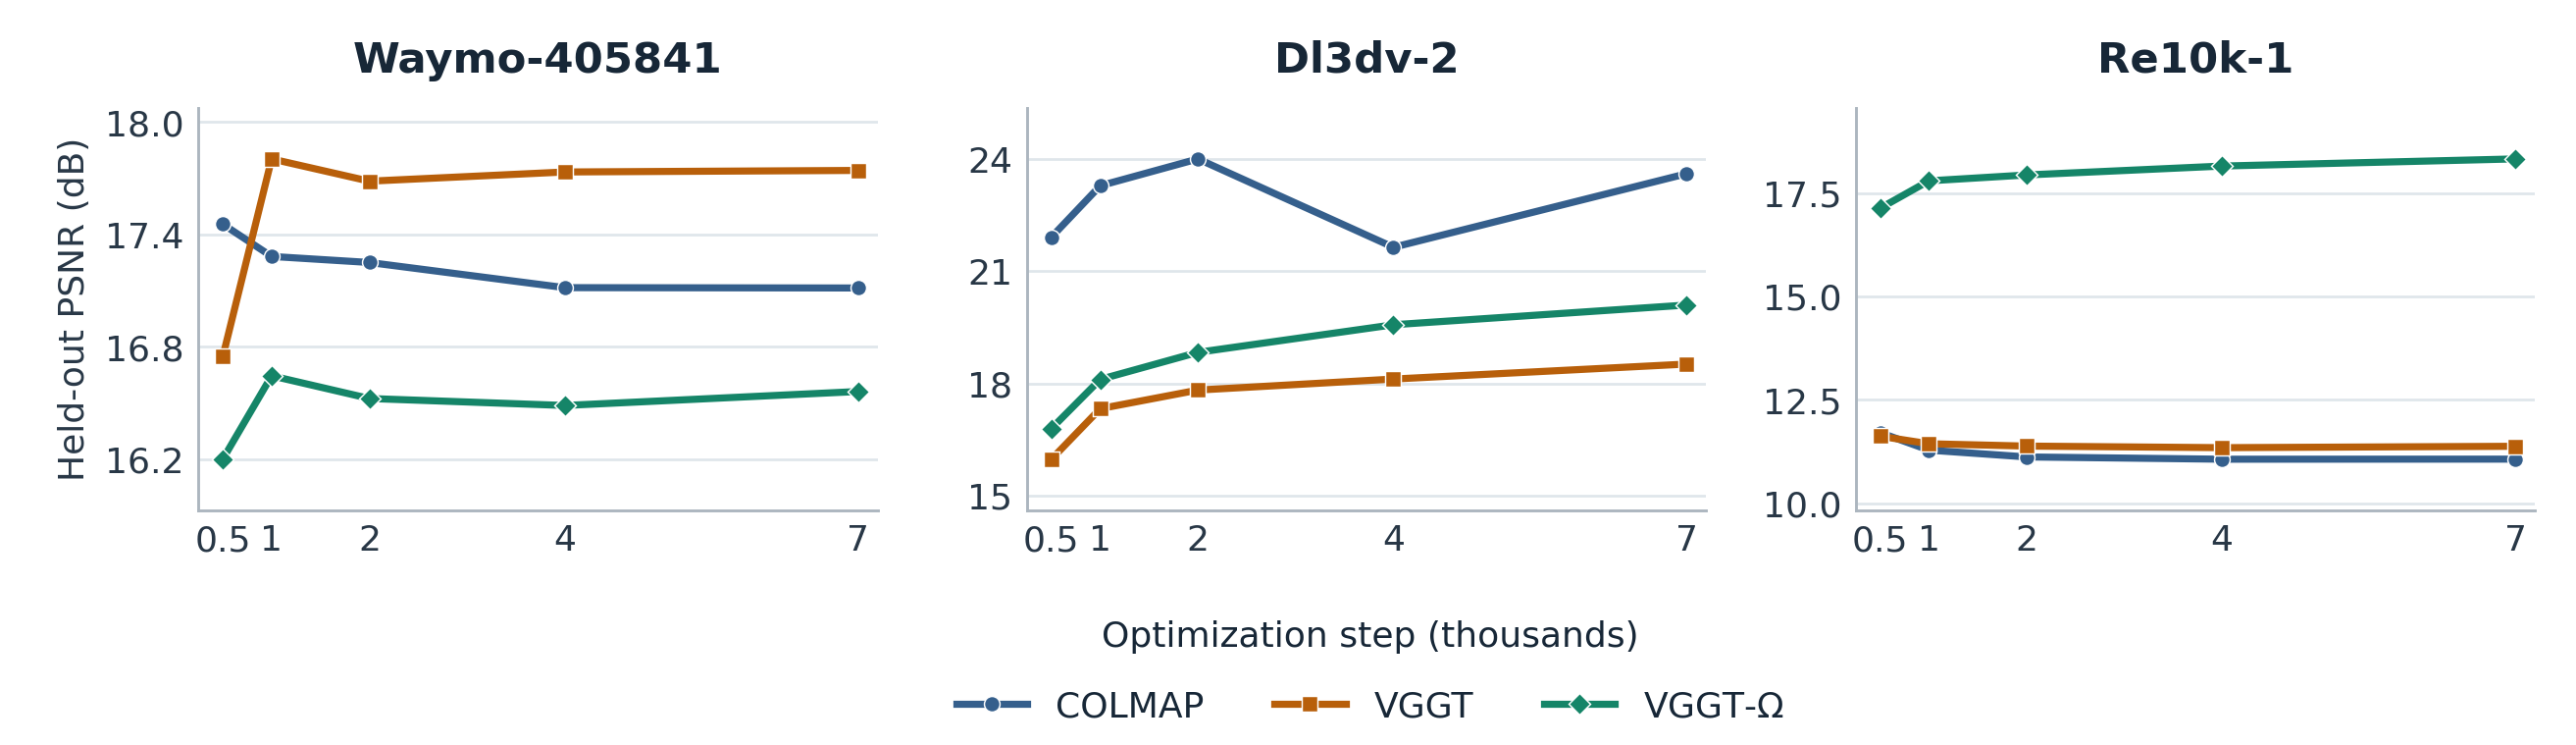
\includegraphics[width=0.94\textwidth]{convergence.png}
  \caption{Dense-view PSNR over the same five checkpoint steps. Several conditions reach their best measured test PSNR before the fixed endpoint.}
  \label{fig:dense_convergence}
\end{figure*}

\paragraph{Initialization cost.}
VGGT-$\Omega$ initializes in 36--42~s and has the shortest end-to-end runtime on all three sequences (Table~\ref{tab:dense}). It is 2.1--2.9$\times$ faster to initialize than VGGT and 9.7--22.3$\times$ faster than our COLMAP configuration. For context, COLMAP uses 8 CPU workers for Waymo and RealEstate10K and 4 for DL3DV. The Waymo matcher uses a 200-image block for 174 input frames to avoid a repeated multi-block failure, and the other scenes use blocks of 50. Earlier camera settings registered only 107 of 174 Waymo views and 66 of 244 RealEstate10K views. Every final COLMAP run registers all training frames. These timing comparisons describe complete working configurations, including their different neural resolutions and SfM settings.

\paragraph{Reconstruction quality.}
On DL3DV, COLMAP leads all quality metrics and has a 3.51~dB PSNR margin over the next best method. Its renders preserve foreground contours and the fa\c{c}ade more clearly (Fig.~\ref{fig:dense_qual}). On RealEstate10K, VGGT-$\Omega$ improves PSNR by 6.95~dB over VGGT and better preserves furniture contours and image borders. On Waymo, VGGT reaches the highest PSNR and SSIM, while COLMAP has better LPIPS and smaller center error. One aligned trajectory score therefore explains only part of the quality ranking.

\paragraph{Convergence and resource use.}
DL3DV's neural initializers improve through all reported checkpoints. COLMAP peaks at 24.00~dB at step 2,000, dips to 21.64~dB at 4,000, then recovers to 23.61~dB (Fig.~\ref{fig:dense_convergence}). RealEstate10K's VGGT-$\Omega$ gains 1.19~dB between steps 500 and 7,000. The nine trained scenes yield 389,467 to 721,872 Gaussians and peak allocated training memory of 0.66--1.30~GiB. Differences in initialization cost are larger than training-time differences within each scene.

\subsection{Part 2: Full versus sparse unposed input}
\label{sec:part2}

\begin{table*}[!t]
  \centering\small
  \begin{tabular}{llrrrrrrr}
    \toprule
    Scene & Input & PSNR (dB) $\uparrow$ & SSIM $\uparrow$ & LPIPS $\downarrow$ & Paired ATE $\downarrow$ & Init. (s) & Train (s) & Total (s) \\
    \midrule
    Waymo & Full & \textbf{17.689} & \textbf{0.6542} & 0.5204 & 0.95649 & 661.5 & 563.8 & 1322.4 \\
          & Sparse & 16.726 & 0.5971 & \textbf{0.4574} & \textbf{0.72937} & 109.0 & 703.7 & 901.2 \\
    DL3DV & Full & \textbf{18.609} & \textbf{0.5142} & \textbf{0.1843} & 0.03790 & 836.5 & 308.1 & 1198.5 \\
          & Sparse & 15.479 & 0.4559 & 0.2572 & \textbf{0.02903} & 79.3 & 160.0 & 273.7 \\
    RealEstate10K & Full & \textbf{11.364} & \textbf{0.2910} & \textbf{0.3957} & 0.02902 & 925.9 & 474.8 & 1459.4 \\
                  & Sparse & 11.234 & 0.2751 & 0.4055 & \textbf{0.02643} & 69.3 & 321.9 & 427.3 \\
    \bottomrule
  \end{tabular}
  \caption{Part 2 at 7,000 steps. Paired ATE evaluates both models on the same sparse training camera IDs. Initialization and training columns are the internal stage timers. Total sums initialization, training, rendering, and evaluation subprocess wall-clock times, including their startup and I/O.}
  \label{tab:sparse}
\end{table*}

\begin{figure*}[!t]
  \centering
  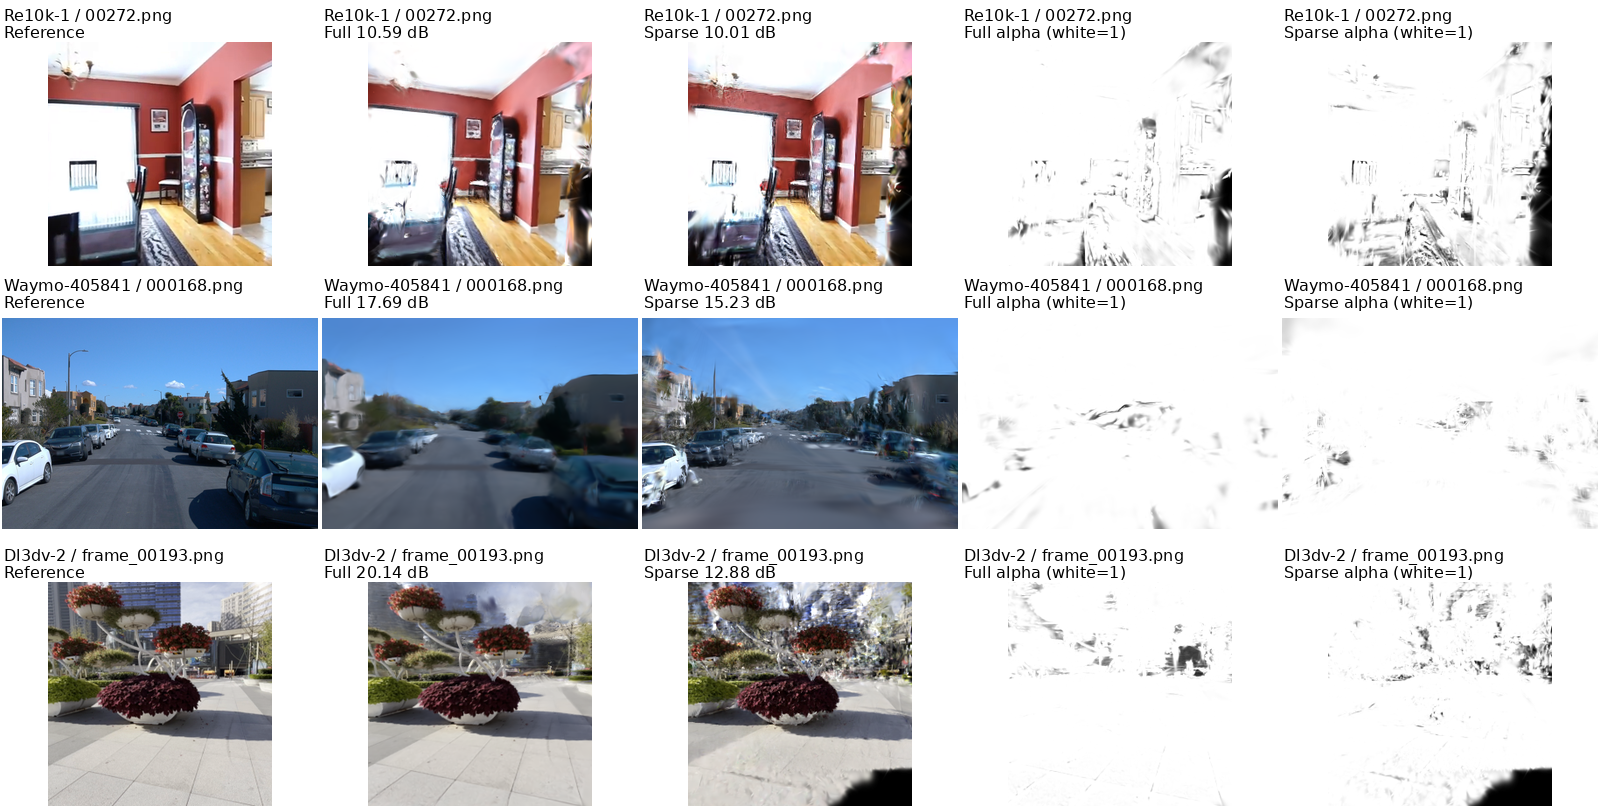
\includegraphics[width=0.94\textwidth]{failure_cases.png}
  \caption{Within each scene, the held-out view with the largest full-minus-sparse PSNR gap. The last two columns show accumulated alpha as projected support (white is opaque). The view selection illustrates failure modes, and the quantitative comparison evaluates every held-out view.}
  \label{fig:sparse_failures}
\end{figure*}

\ifpartthreeevidence\partthreeassets\fi

\paragraph{Rendering and runtime.}
Full input improves average PSNR and SSIM on all three sequences. The largest PSNR change is 3.13~dB on DL3DV. Waymo shows a metric split: full achieves higher PSNR on 24 of 25 views, while sparse achieves lower LPIPS on all 25 views. With fewer cameras, initialization falls from 661--926~s to 69--109~s. The sparse Waymo model takes longer to optimize and finishes with about 839,000 Gaussians, compared with 484,000 in the full condition. The sparse total time is nevertheless lower in each scene (Table~\ref{tab:sparse}).

\paragraph{Pose and visibility.}
Sparse has lower center ATE on the shared camera IDs, but on Waymo its mean orientation discrepancy increases from $1.05^\circ$ to $2.21^\circ$. Re10k's independent full and sparse VGGT initializations both estimate focal lengths approximately 20\% above the supplied reference. Figure~\ref{fig:sparse_failures} shows a cabinet boundary distorted in both Re10k conditions and fragmented foliage and dark ground regions in sparse DL3DV. The mean fraction of test pixels with alpha at least 0.9 falls from 95.98\% to 92.29\% in DL3DV and from 87.27\% to 83.69\% in Re10k. Alpha measures projected support. Incorrect opaque structures can still have high accumulated alpha.

\paragraph{Convergence and replay.}
Sparse Re10k and Waymo peak early in the observed checkpoints, while sparse DL3DV's highest sampled PSNR exceeds the last checkpoint by 0.63~dB. The \href{https://github.com/MoliaiELS/CV_Project4/blob/main/results/part2_supplement_v1/figures/convergence_all_metrics.png}{archived curves} retain all five measurements per metric. Replay of all three archived Part 1 VGGT checkpoints on the course GPU reproduces their archived final PSNR at six decimal places. Those full results are within 0.09~dB of the independently trained Part 2 full runs. The primary contrast uses the native Part 2 pairs.

\subsection{Part 3: Generative reconstruction}
\label{sec:part3}
\ifpartthreeevidence
\partthreeresults
\else
The evaluation compares the initial sparse checkpoint $M_0$ and the Gaussian scenes from every round with a real-only continuation at the same step. Raw held-out renders use the fixed Part 2 test cameras. The restored virtual views and confidence maps describe where the method applies new supervision; the held-out comparison tests whether the updates generalize.

\emph{Part 3 evidence to be loaded from verified run artifacts before submission.}
\fi
